\chapter{Software on PR2}
\section{pr2\_core}
There is a core set of code that always runs by default on the robot.  This includes:
\begin{description}
\item[roscore]
\item[diagnostics logging] to /hwlogs
\item[web interface] which exports a set of webpages at XXX for basic robot control
\item[pr2\_etherCAT]
\item[power\_board]
\item[battery\_monitor]
\item[sensor drivers]
This list is controlled by the launch files in XXX, which are used by rosinit on startup, and any time that the robot needs to "reset" to the default state (or when a developer wants to change one of those components)
\end{description} 
\section{pr2\_dashboard}
pr2\_dashboard, Figure~\ref{fig:dashboard}, is a GUI for debugging and controlling low-level state of the PR2. The dashboard displays the diagnostic, 
circuit breaker, runstop, and battery status.
\begin{figure}[h]
\centering
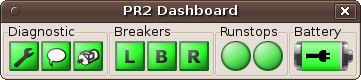
\includegraphics[scale=0.5]{pr2_dashboard.png}
\caption{The PR2 dasboard.}
\label{fig:dashboard}
\end{figure}
\begin{description}
\item[Diagnostic Status] The state of the robot is shown by the diagnoctic indicators in the pr2\_dashboard. \\

    \newcolumntype{S}{>{\centering\arraybackslash} m{.9cm} }%
    \begin{tabular}{m{6cm}SSSS}
    Component & OK & Warn & Error & Stale\\
    &&&&\\
    Diagnostics: Clicking pops up the Robot Monitor & 
\includegraphics[scale=0.5]{diag_error.png}&
\includegraphics[scale=0.5]{diag_warn.png}&
                                                      
\includegraphics[scale=0.5]{diag_ok.png}&
\includegraphics[scale=0.5]{diag_stale.png}\\
    &&&&\\
    Rosout: Clicking pops up rxconsole & 
\includegraphics[scale=0.5]{rosout_error.png}&
\includegraphics[scale=0.5]{rosout_warn.png}&
                                        
\includegraphics[scale=0.5]{rosout_ok.png}&
\includegraphics[scale=0.5]{rosout_stale.png}\\
    &&&&\\
    Motors: Clicking allows you to halt or reset motors & 
\includegraphics[scale=0.5]{motor_error.png}& N/A &
                                                          
\includegraphics[scale=0.5]{motor_ok.png}&
\includegraphics[scale=0.5]{motor_stale.png}\\
   \end{tabular}

\item[Circuit Breaker Status] The circuit breakers are labeled L/B/R, which stand for Left Arm, Base/Spine, and Right Arm. 
Each breaker can be in one of four states, and clicking on any of the breakers will pop up a menu allowing you to change 
the state of one or all of them:
\begin{figure}[h]
\centering
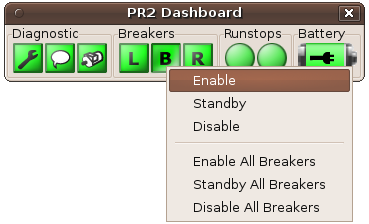
\includegraphics[scale=0.5]{breakers_menu.png}
\caption{The circuit breaker options menu.}
\label{fig:dashboard}
\end{figure}



\item[Runstop Status]

\item[Battery Status]

\end{description}

\section{Apps}
This section should contain a list of all the top-level useful apps shipping with the PR2.  We need some template for structuring this data, and ideally this documentation would be pulled from the apps themselves.

\subsection{joystick\_teleop or replacement}
\subsection{...}
\section{Data and robot configuration}
\subsection{Robot description}
\subsection{pr2.launch and pr2.urdf}
Local versions of launch file and urdf that live in /etc/pr2/ and can be calibrated, changed to accomodate new sensors or robot changes, etc.

Describe API of full robot here (what topics, services, etc. the PR2 has when it's up)
\subsubsection{Integrating calibration data}
Basically, over-write /etc/pr2/pr2.launch
